\documentclass{article}

% Language setting
% Replace `english' with e.g. `spanish' to change the document language
\usepackage[english]{babel}

% Set page size and margins
% Replace `letterpaper' with`a4paper' for UK/EU standard size
\usepackage[a4paper,top=2cm,bottom=2cm,left=3cm,right=3cm,marginparwidth=1.75cm]{geometry}

% Useful packages
\usepackage{amsmath}
\usepackage{graphicx}
\usepackage{listings}
\usepackage{xcolor}
\usepackage[colorlinks=true, allcolors=blue]{hyperref}

\usepackage{algorithm, algpseudocode}
\usepackage{csquotes}
\usepackage{subfig}

\definecolor{codegreen}{rgb}{0,0.6,0}
\definecolor{codegray}{rgb}{0.5,0.5,0.5}
\definecolor{codepurple}{rgb}{0.58,0,0.82}
\definecolor{backcolour}{rgb}{0.95,0.95,0.92}

\lstdefinestyle{mystyle}{
    backgroundcolor=\color{backcolour},   
    commentstyle=\color{codegreen},
    keywordstyle=\color{magenta},
    numberstyle=\tiny\color{codegray},
    stringstyle=\color{codepurple},
    basicstyle=\ttfamily\footnotesize,
    breakatwhitespace=false,         
    breaklines=true,                 
    captionpos=b,                    
    keepspaces=true,                 
    numbers=left,                    
    numbersep=5pt,                  
    showspaces=false,                
    showstringspaces=false,
    showtabs=false,                  
    tabsize=2
}

\lstset{style=mystyle}
\newcommand{\code}[1]{\lstinline|#1|}
\setlength\parindent{0pt}

\title{Homework 5\\CS3316 Reinforce learning}
\author{Ng Tze Kean\\Student number: 721370290002}

\begin{document}
\maketitle

\begin{titlepage}
\end{titlepage}

\section*{A3C}

Training agents through reinforcement learning can be a slow process,
especially when dealing with complex environments. Traditional methods often
rely on a single agent interacting with the environment, limiting exploration
and hindering learning speed. The Asynchronous Advantage Actor-Critic (A3C)
algorithm addresses these limitations by introducing several innovative
approaches, making it a powerful technique in Deep Reinforcement Learning.

A key strength of A3C lies in its use of parallelization. Instead of a single
agent, A3C employs multiple agents that explore the environment concurrently.
This significantly speeds up the learning process compared to a single agent
approach. Imagine a team of agents simultaneously exploring a maze; they can
collectively gather information and learn the optimal path much faster than a
single agent navigating alone.

Furthermore, A3C leverages a powerful combination of two neural networks: the
actor and the critic. The actor network acts as the decision-maker, selecting
actions for the agent within the environment. The critic network, on the other
hand, plays the role of an evaluator, assessing the chosen actions and the
resulting rewards or penalties. By combining these two networks, A3C gains a
deeper understanding of the environment. It not only learns which actions to
take, but also how valuable those actions are in the long run.

Another key feature of A3C is its use of asynchronous updates. As each agent
gathers experiences, it asynchronously updates a central "global network." This
allows for faster learning compared to waiting for a single agent to complete
its exploration and update the network. Imagine multiple students working on a
group project, each contributing their findings and updates to a central
document simultaneously. This collaborative learning approach significantly
reduces the overall learning time.

The combined effect of these approaches makes A3C a standout method in
reinforcement learning. Parallel exploration and asynchronous updates
significantly accelerate the learning process. Additionally, the use of
multiple agents encourages broader exploration of the environment, reducing
bias and leading to a more robust understanding of the available actions.
Finally, A3C's ability to leverage distributed computing resources makes it
well-suited for large-scale systems and complex environments.

\begin{figure}[h]
    \centering
    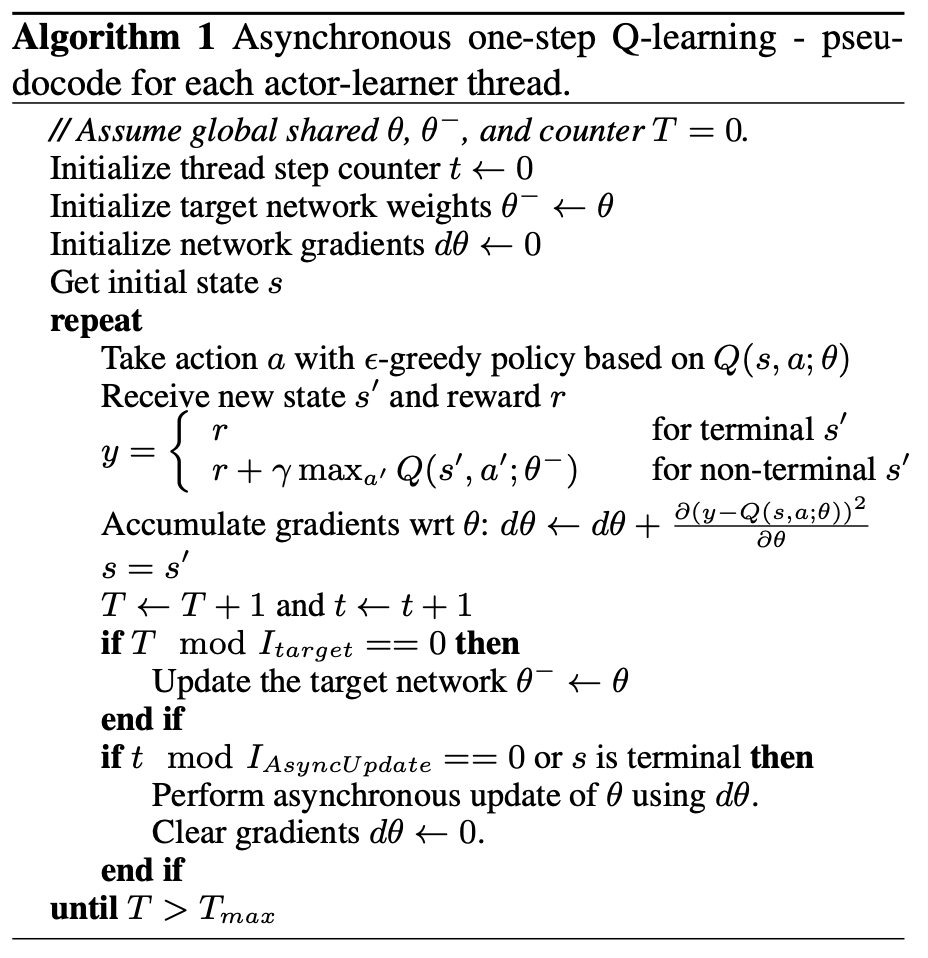
\includegraphics[width=0.6\textwidth]{a3c.png}
    \caption{A3C pseudo code}
\end{figure}

\section*{DDPG}

Deep Deterministic Policy Gradient (DDPG) is a powerful algorithm within Deep
Reinforcement Learning, particularly adept at handling environments with
continuous action spaces. Unlike traditional methods that require the agent to
strictly follow a specific policy during training, DDPG leverages a technique
called off-policy learning. This allows the agent to learn from a broader range
of experiences, even those not generated by the current policy, leading to more
efficient learning.

A key strength of DDPG lies in its use of actor-critic methods. Similar to A3C,
DDPG employs two neural networks: the actor and the critic. The actor network
acts as the agent's brain, selecting actions within the environment. The critic
network, on the other hand, plays the role of a reviewer, evaluating the chosen
actions and their resulting rewards or penalties. This collaborative approach
allows DDPG to not only learn which actions to take, but also how valuable
those actions are in the long run.

To ensure stable learning during the training process, DDPG introduces a unique
concept: separate target networks for both the actor and the critic. These
target networks are periodically updated with the weights from the main
networks. This separation helps to stabilize the learning process and prevent
the networks from becoming overly sensitive to changes in the data.

Furthermore, DDPG utilizes a technique called experience replay. The agent
stores past experiences in a replay buffer, allowing it to revisit and learn
from a diverse set of data points during training. This not only improves
learning efficiency but also helps to prevent the networks from overfitting on
specific scenarios within the environment.

DDPG's ability to handle high-dimensional state spaces, where the environment
can be described by many variables, and continuous action spaces, where actions
have real-world consequences, makes it particularly suitable for complex tasks.
It has achieved success in various applications, particularly in robotic
control, where robots need to learn precise and continuous movements to perform
various tasks. Additionally, DDPG excels in continuous control problems, such
as controlling a car or a drone, where actions directly impact the physical
world.

\begin{figure}[h]
    \centering
    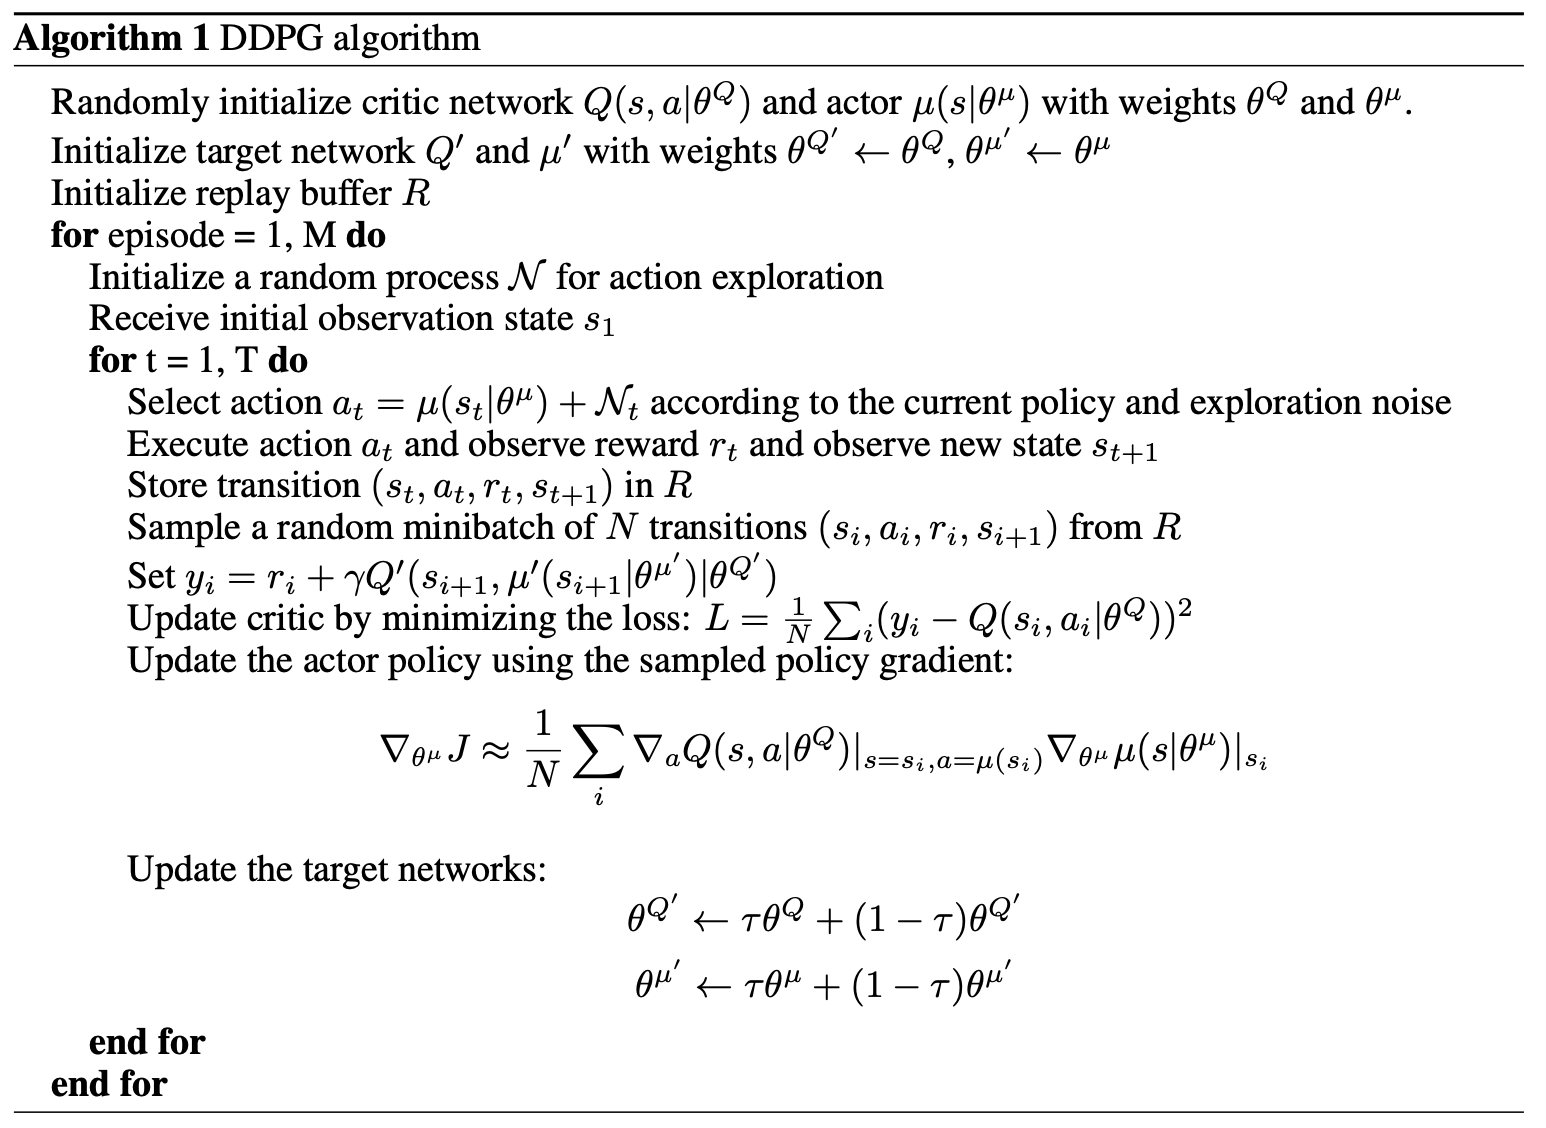
\includegraphics[width=0.6\textwidth]{ddpg.png}
    \caption{A3C pseudo code}
\end{figure}

\section*{Architecture}

The lab uses the Pendulum environment form OpenAI and the 2 agents are
implemented in python3. We fix the other hyperparameters such as the number of
hidden layers and the number of episodes. We then train the agents and compare
the number of steps to reach convergence and the overall maximum reward of
the agent.

We set the hidden layer for the neural network to be 64, and we try to keep
all other

\section*{Results}

\begin{figure}[h]%
    \centering
    \subfloat[\centering A3C]{{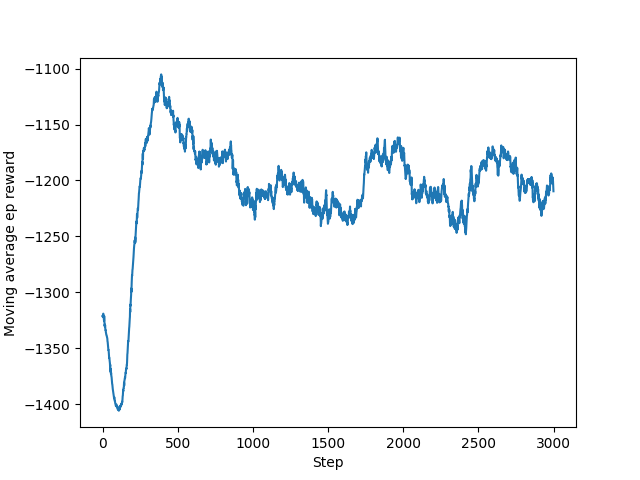
\includegraphics[width=6cm]{a3c_results.png} }}%
    \qquad
    \subfloat[\centering DDPG]{{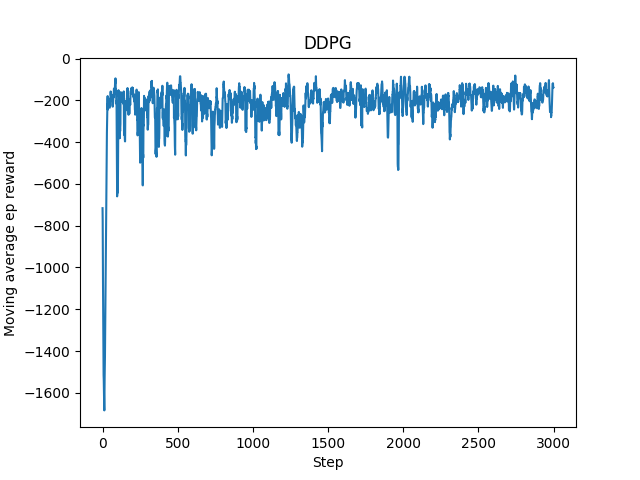
\includegraphics[width=6cm]{ddpg_results.png} }}%
    \caption{Results of both methods}%
    \label{fig:example}%
\end{figure}

We note that the training for A3C is much faster than DDPG. The A3C agent runs
the episodes in parallel and updates the global network asynchronously. This is
different from DDPG where the agent runs the episodes sequentially and updates
the network after each episode. This makes A3C much faster than DDPG in terms
of training. The overall time taken to train the A3C was about 1/5 the time
taken to train the DDPG agent.

However, as we can see from the images above the DDPG agent has a much higher
reward than the A3C agent. This is because the DDPG agent is able to learn the
optimal policy much better than the A3C agent. The graph of the DDPG agent is
also generally more stable than the A3C agent. We can see that once the DDPG
agent has converged, it is able to maintain a high reward throughout the training
process. This is not the case for the A3C agent which has a more erratic reward
graph.

\section*{Conclusion}

Overall we can see that A3C tends to favour exploration over expliotation with
its parallel exploration and asynchronous updates. This makes it faster than
DDPG but it is not able to learn the optimal policy as well as DDPG. This is
due to insufficient expliotation by the agent during the training. DDPG on the
other hand is able to learn the optimal policy much better than A3C from its
off policy learning and experience replay. But this comes at a cost of longer
training time.

\end{document}